\chapter{最基础的概念}
\label{chap:01}

\begin{chapteropening}
望远镜收到的“光”在数据里到底变成了什么？一台望远镜不会直接保存一束连续电磁波，也不会直接保存一张已经有物理解释的图像。它最终保存的是计数、时间、通道、位置和质量标记。

最基础的语言从这里开始：光可以用电场描述；探测器通常只留下强度和光子计数；事件表、Poisson 噪声和几个数量级共同决定公式里的基本单位和基本数据字段。
\end{chapteropening}

\section{望远镜真正记录了什么}
\label{sec:1-language}

最底层的数据不是“图像”，而是一条条事件。一次光子探测可以记为
\begin{equation}
  e_j=(t_j,\bm{r}_j,\nu_j,p_j,w_j).
  \label{eq:event-row}
\end{equation}
\begin{formulaexplain}
\(e_j\) 表示第 \(j\) 条探测事件；\(t_j\) 是时间戳，\(\bm r_j\) 是接收位置或像素，\(\nu_j\) 是频率通道，\(p_j\) 是偏振或电子学通道，\(w_j\) 是质量权重。这条式子的意义是把一次光子点击写成可分析的数据行。
\end{formulaexplain}
这里 \(j\) 是事件编号；\(t_j\) 是到达时间，单位通常是秒、纳秒或皮秒；\(\bm r_j\) 表示接收位置，可以是望远镜编号、探测器像素或阵列坐标；\(\nu_j\) 是频率或光谱通道，单位 Hz 或通道号；\(p_j\) 是偏振、探测器或电子学通道标签；\(w_j\) 是权重或质量标记，可以记录背景概率、坏像素、死时间附近事件、云层筛选或效率修正。

这行式子不是为了复杂化数据，而是为了提醒我们：同一批光子可以被投影成很多不同产品。若按天空位置分箱，就得到图像；按频率分箱，就得到光谱；按时间分箱，就得到光变曲线；按偏振通道组合，就得到偏振量。每一次投影都会保留一部分信息，也会丢掉一部分信息。后面的章节之所以反复回到事件表，是因为许多快速变化、通道相关和时间相关问题一旦先被平均，就很难再恢复。

\section{光为什么既有波的语言也有计数的语言}
\label{sec:1-light}

在一个足够窄的频率通道里，光可以先近似看成单色电磁波。真实振荡的是电场，例如
\begin{equation}
  E(t)=E_0\cos(\omega t+\phi),
  \qquad \omega=2\pi\nu .
  \label{eq:monochromatic-field}
\end{equation}
\begin{formulaexplain}
\(E(t)\) 是时刻 \(t\) 的真实电场；\(E_0\) 是振幅；\(\omega\) 是角频率；\(\nu\) 是普通频率；\(\phi\) 是相位。它说明单色光的波动信息首先存在于电场的快速振荡中。
\end{formulaexplain}
\(E_0\) 是电场振幅，\(\omega\) 是角频率，\(\nu\) 是频率，\(\phi\) 是相位。可见光频率约为 \(4\times10^{14}\) 到 \(8\times10^{14}\,{\rm Hz}\)，一个光学周期只有几飞秒。普通天文探测器的响应远慢于这个周期，因此它通常不会逐周期记录 \(E(t)\) 的正负振荡。

为了同时表示振幅和相位，常把电场写成复振幅：
\begin{equation}
  \mathcal{E}=E_0e^{i\phi},
  \qquad
  E(t)=\operatorname{Re}\!\left[\mathcal{E}e^{i\omega t}\right].
  \label{eq:phasor-field}
\end{equation}
\begin{formulaexplain}
\(\mathcal E\) 是复振幅；\(|\mathcal E|=E_0\) 给出振幅；\(\arg\mathcal E=\phi\) 给出相位；\(\operatorname{Re}\) 表示取实部。这条式子把振幅和相位合进一个复数，方便讨论干涉。
\end{formulaexplain}
\(\mathcal E\) 的模 \(|\mathcal E|=E_0\) 表示振幅，辐角 \(\arg\mathcal E=\phi\) 表示相位。可以把它想成一支旋转箭头：长度是振幅，方向是相位。相位的单位是弧度，本质上是无量纲角变量。

探测器真正留下的通常是强度或光子数。把光学快速振荡在探测器响应时间内平均后，强度近似正比于电场平方：
\begin{equation}
  I\propto \langle E^2(t)\rangle_{\rm det}
  \propto |\mathcal{E}|^2 .
  \label{eq:intensity-from-field}
\end{equation}
\begin{formulaexplain}
\(I\) 是探测到的强度；\(\langle\cdots\rangle_{\rm det}\) 表示在探测器响应时间内平均；\(|\mathcal E|^2\) 是复振幅模平方。它说明探测器通常记录能量相关量，而不是电场的瞬时正负振荡。
\end{formulaexplain}
物理上，这条式子说的是：探测器吸收能量，能量密度和场的平方有关。因此相位本身通常不会被直接记录；它只能通过干涉、调制或后续的相关测量间接影响强度数据。

最简单的干涉来自两束光的电场相加。若两束光进入同一探测器，先相加的是电场，后平方的是强度：
\begin{equation}
  I\propto |\mathcal{E}_1+\mathcal{E}_2|^2
  =
  |\mathcal{E}_1|^2+|\mathcal{E}_2|^2
  +2\,\operatorname{Re}(\mathcal{E}_1\mathcal{E}_2^\ast).
  \label{eq:two-beam-interference}
\end{equation}
\begin{formulaexplain}
\(\mathcal E_1,\mathcal E_2\) 是两束光的复振幅；前两项是各自强度；\(2\operatorname{Re}(\mathcal E_1\mathcal E_2^\ast)\) 是交叉干涉项；星号表示复共轭。这条式子说明普通干涉来自电场先相加再取模平方。
\end{formulaexplain}
前两项是两束光各自的强度；最后一项是干涉项。如果写成 \(\mathcal E_1=E_1e^{i\phi_1}\)、\(\mathcal E_2=E_2e^{i\phi_2}\)，干涉项就是 \(2E_1E_2\cos(\phi_1-\phi_2)\)。相位差接近 0 时相长，接近 \(\pi\) 时相消。后面的干涉测量章节会在这个基本事实上继续展开。

天文学里最常见的几何相位来自路程差：
\begin{equation}
  \Delta\phi=\frac{2\pi}{\lambda}\,\bm B\cdot\bm s .
  \label{eq:geometric-phase}
\end{equation}
\begin{formulaexplain}
\(\Delta\phi\) 是几何相位差；\(\lambda\) 是波长；\(\bm B\) 是两接收点的基线；\(\bm s\) 是源方向单位向量；\(\bm B\cdot\bm s\) 是路程差。这条式子把望远镜几何换成光学相位。
\end{formulaexplain}
\(\bm B\) 是两处接收点之间的基线向量，单位厘米；\(\bm s\) 是源方向单位向量；\(\lambda\) 是波长。点积 \(\bm B\cdot\bm s\) 是沿源方向的路程差，\(2\pi/\lambda\) 把长度换成相位。多走一个波长，相位就多 \(2\pi\)。这条式子只给出最基础的相位语言；两台望远镜之间更完整的空间关系将在第 \ref{chap:05} 章正式定义。

\begin{figure}[tbp]
\centering
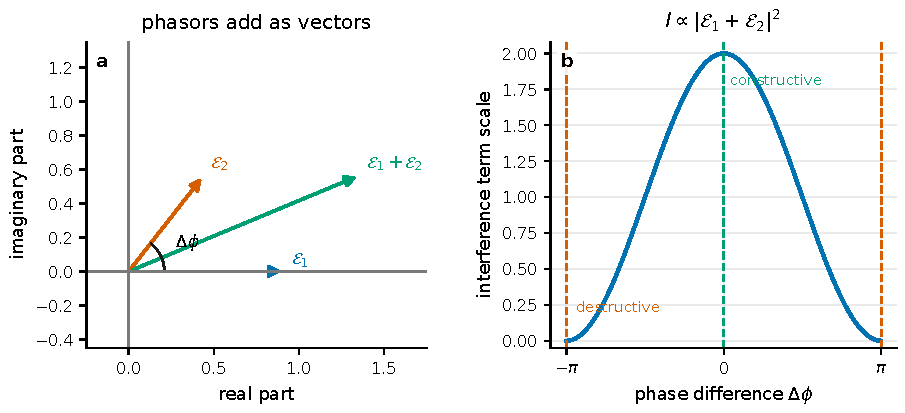
\includegraphics[width=0.86\linewidth]{figures/generated/chapter_01/ch01_phase_interference.pdf}
\caption{复振幅和两束光干涉的基本图像。复振幅像箭头一样相加；探测器看到的是合成箭头长度的平方。相位差决定干涉项是正、负还是被平均掉。}
\label{fig:ch01-phase-interference}
\end{figure}

\section{为什么计数会有噪声}
\label{sec:1-counting}

探测器把光变成离散点击以后，最基本的随机量就是某个时间窗内的计数。选定时间 bin 宽度 \(\Delta t\)，若平均光子到达率为 \(R_\gamma\)，则平均计数为
\begin{equation}
  \mu=R_\gamma\Delta t .
  \label{eq:mean-count}
\end{equation}
\begin{formulaexplain}
\(\mu\) 是一个时间 bin 中的平均光子数；\(R_\gamma\) 是平均光子到达率；\(\Delta t\) 是时间 bin 宽度。它把连续的光子率换成离散计数模型中的平均数。
\end{formulaexplain}
\(R_\gamma\) 的单位是 \({\rm s^{-1}}\)，\(\Delta t\) 的单位是秒，\(\mu\) 是无量纲平均光子数。若 \(\Delta t=1\,{\rm ms}\)、\(R_\gamma=10^5\,{\rm s^{-1}}\)，则每个 bin 平均有 \(\mu=100\) 个光子。

这里的“平均”很重要。它不是说每个 \(1\,{\rm ms}\) 时间窗都会精确收到 100 个光子，而是说把很多个相同条件下的时间窗放在一起平均，结果接近 100。真实事件表里，有的 bin 会多几个，有的 bin 会少几个。即使天体亮度、望远镜面积和探测效率都保持不变，这种涨落也不会消失，因为探测器记录的是一次次离散点击。

先看最简单的情形：在这个短时间窗内，光子没有互相“约好”一起到达，也没有因为前一个光子刚到过就避开下一个光子。换句话说，给定平均到达率以后，不同极短时间片里的点击可以先近似看成独立事件。把一个时间 bin 切成 \(M\) 个很短的小格，每个小格宽度为 \(\delta t=\Delta t/M\)。若 \(\delta t\) 足够短，一个小格里要么没有光子，要么有一个光子，出现光子的概率近似为
\[
  p=R_\gamma\delta t .
\]
这个近似的意思很物理：光子率越高，小格越长，看到一次点击的机会越大；但只要小格足够短，两个光子挤进同一个小格的概率就可以忽略。

在这个离散小格图像里，\(N\) 个光子就是 \(M\) 个小格中恰好有 \(N\) 个小格发生点击。若各小格彼此独立，计数先服从二项分布：
\begin{equation}
  P_M(N)=\binom{M}{N}p^N(1-p)^{M-N},
  \qquad Mp=R_\gamma\Delta t=\mu .
  \label{eq:poisson-from-binomial}
\end{equation}
\begin{formulaexplain}
\(P_M(N)\) 是切成 \(M\) 个小格后数到 \(N\) 个光子的概率；\(p\) 是每个小格发生一次点击的概率；\(\binom{M}{N}\) 是选择哪些小格发生点击的方式数；\(Mp=\mu\) 是整个 bin 的平均计数。
\end{formulaexplain}
现在让小格越来越细：\(M\) 很大，\(p\) 很小，但总平均数 \(Mp=\mu\) 保持不变。二项分布就在这个极限下变成 Poisson 分布。换句话说，Poisson 过程描述的不是“完全没有物理原因的随机”，而是没有额外记忆、没有互相排斥、没有互相吸引的一串稀疏独立到达。

因此，如果光子在给定平均率下彼此独立到达，计数服从
\begin{equation}
  P(N)=e^{-\mu}\frac{\mu^N}{N!},
  \qquad
  \operatorname{Var}(N)=\mu .
  \label{eq:poisson}
\end{equation}
\begin{formulaexplain}
\(P(N)\) 是数到 \(N\) 个光子的概率；\(\mu\) 是平均计数；\(N!\) 给出离散事件排列的归一化；\(\operatorname{Var}(N)\) 是方差。它说明独立到达的光子具有均值等于方差的 shot noise。
\end{formulaexplain}
这条式子的每一部分都有直观含义。因子 \(e^{-\mu}\) 来自“很多小格都没有点击”的总概率；\(\mu^N\) 表示平均计数越大，出现 \(N\) 次点击的权重越高；\(N!\) 则去掉了点击先后顺序的重复计数，因为一个时间 bin 只关心总数 \(N\)，不关心这 \(N\) 次点击在公式展开里被怎样排序。

噪声也可以从这个小格图像看出来。每个小格都是一次小小的随机试验，实际点击数不可能每个 bin 都精确等于平均值。独立随机量相加时，平均数相加，方差也相加；在极小概率极限下，每个小格贡献的方差近似等于它的平均贡献，全部加起来就得到 \(\operatorname{Var}(N)=\mu\)。因此标准差是 \(\sqrt{\mu}\)，相对 shot noise 是 \(1/\sqrt{\mu}\)。当 \(\mu=10^4\) 时，相对涨落约 \(1\%\)；当 \(\mu=1\) 时，离散计数本身就是主导噪声。

这就是后文很多误差估计的起点。只要在固定时间、固定通道、固定选择条件下数光子，就必须先问平均计数是多少，以及 Poisson 噪声有多大。若源本身在变、背景在变、探测器有死时间，或事件之间并不独立，就要在后续章节中把这些效应加入模型。

\begin{figure}[tbp]
\centering
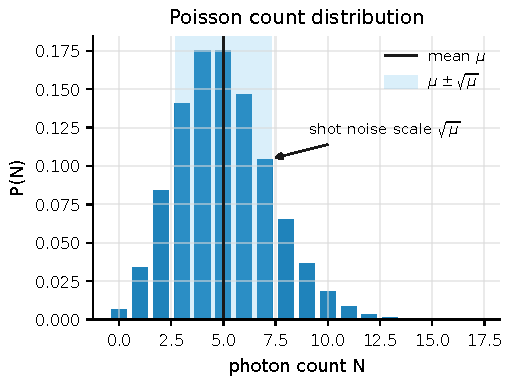
\includegraphics[width=0.86\linewidth]{figures/generated/chapter_01/ch01_photon_count_statistics.pdf}
\caption{Poisson 计数分布的基本形状。平均计数为 \(\mu\) 时，方差也是 \(\mu\)，shot noise 的尺度为 \(\sqrt{\mu}\)。}
\label{fig:chapter-01-02}
\end{figure}

\section{几个必须先记住的数量级}
\label{sec:1-scales}

第一，时间误差可以换成光程误差：
\begin{equation}
  \Delta \ell=c\,\Delta t .
  \label{eq:path-time}
\end{equation}
\begin{formulaexplain}
\(\Delta\ell\) 是光程误差；\(c\) 是光速；\(\Delta t\) 是计时误差或延迟误差。这条式子把时间同步精度直接换算成空间尺度。
\end{formulaexplain}
\(c\simeq3.0\times10^{10}\,{\rm cm\,s^{-1}}\) 是光速。\(1\,{\rm ps}\) 对应约 \(3.0\times10^{-2}\,{\rm cm}\)，\(1\,{\rm ns}\) 对应约 \(30\,{\rm cm}\)。所以只要讨论快速计时、几何延迟或两个站点的同步，时间单位马上会变成空间尺度。

第二，光子能量由频率或波长决定：
\begin{equation}
  E_\gamma=h\nu=\frac{hc}{\lambda}.
  \label{eq:photon-energy}
\end{equation}
\begin{formulaexplain}
\(E_\gamma\) 是单个光子的能量；\(h\) 是 Planck 常数；\(\nu\) 是频率；\(c\) 是光速；\(\lambda\) 是波长。它说明高频短波长光子携带更高能量。
\end{formulaexplain}
\(h\) 是 Planck 常数。蓝光光子比红光光子能量高；同样的能量流量，在红光中对应更多光子。把能量流量换成光子率时，必须除以 \(E_\gamma\)。

第三，带宽可以在频率和波长之间换算。对窄带近似，
\begin{equation}
  \Delta\nu\simeq \frac{c\,\Delta\lambda}{\lambda^2}.
  \label{eq:bandwidth-conversion}
\end{equation}
\begin{formulaexplain}
\(\Delta\nu\) 是频率带宽；\(\Delta\lambda\) 是波长带宽；\(\lambda\) 是中心波长；\(c\) 是光速。它给出窄带近似下波长分辨率和频率分辨率的换算。
\end{formulaexplain}
\(\Delta\lambda\) 是波长带宽。以 \(\lambda=500\,{\rm nm}\)、\(\Delta\lambda=1\,{\rm nm}\) 为例，\(\Delta\nu\simeq1.2\times10^{12}\,{\rm Hz}\)。后面讨论光谱通道和相干时间时，会反复用到这个换算。

第四，探测到的光子率可以粗略写成
\begin{equation}
  R_\gamma=A\eta\int F_\lambda\frac{\lambda}{hc}\,d\lambda .
  \label{eq:photon-rate}
\end{equation}
\begin{formulaexplain}
\(R_\gamma\) 是探测光子率；\(A\) 是有效收集面积；\(\eta\) 是总效率；\(F_\lambda\) 是谱流量密度；\(\lambda/(hc)\) 把能量流量换成光子数；积分表示对带宽求和。
\end{formulaexplain}
\(A\) 是有效收集面积，单位 \({\rm cm^2}\)；\(\eta\) 是系统总效率；\(F_\lambda\) 是谱流量密度；\(\lambda/(hc)\) 把能量流量换成光子数流量。这个式子告诉我们，目标亮度、望远镜面积、带宽和效率共同决定事件表里到底有多少光子。

\begin{longtable}{p{0.24\linewidth}p{0.30\linewidth}p{0.34\linewidth}}
\toprule
量 & 常见数量级 & 基本意义 \\
\midrule
\(\lambda\) & \(350\,{\rm nm}\) 到 \(1.6\,\mu{\rm m}\) & 观测波长。 \\
\(\nu\) & \(10^{14}\)--\(10^{15}\,{\rm Hz}\) & 光学频率。 \\
\(\Delta t\) & ps 到 s & 时间戳精度、bin 宽或曝光时间。 \\
\(R_\gamma\) & \(<1\) 到 \(10^9\,{\rm s^{-1}}\) & 单通道探测光子率。 \\
\(\mu\) & \(R_\gamma\Delta t\) & 一个 bin 中的平均计数。 \\
\(1/\sqrt{\mu}\) & 从很大到很小 & Poisson 相对噪声。 \\
\(\eta\) & \(0.01\) 到 \(0.5\) & 大气、光学和探测器总效率。 \\
\bottomrule
\end{longtable}
